\chapter{Conclusiones, Limites y Trabajo Futuro}

\section{7.1 Sintesis de resultados frente a la hipotesis}
La hipotesis central de la tesis afirma que una politica de particion heterogenea CPU-GPU, construida a partir de evidencia empirica robusta y optimizacion declarativa, puede mejorar el comportamiento global frente a politicas simples sin perder validez operacional. A la fecha de este borrador, esa hipotesis ya cuenta con sustento parcial fuerte. El pipeline de profiling existe y produce coeficientes admisibles; el ILP supera a baselines \code{all_cpu} y \code{greedy} en el caso smoke consolidado; la solucion puede transformarse en plan, simularse y ejecutarse en runtime; y la version extendida con decisiones duales y prefetching ya ha sido materializada en evidencia controlada.

El resultado mas claro disponible en esta etapa es el cierre del circuito metodologico minimo. La tesis ya puede afirmar que mide, decide, simula y ejecuta. Lo que aun no puede afirmar con igual amplitud es la universalidad de ese comportamiento sobre una matriz multi-servidor y multi-arquitectura estadisticamente amplia. Por ello, la hipotesis debe presentarse en este borrador como fuertemente apoyada en viabilidad metodologica y en evidencia focal, pero pendiente de cierre empirico transversal final.

\section{7.2 Contribuciones metodologicas y de sistemas}
Las contribuciones del trabajo pueden sintetizarse en cuatro niveles complementarios. Primero, se construye un sistema de profiling por capa que integra tiempo, energia, memoria, transferencia y procedencia estructural del grafo bajo un contrato de artefactos reproducible. Segundo, se formula un ILP robusto e interpretable que traduce esa evidencia en una decision binaria ejecutable bajo restricciones de memoria y con soporte para sensibilidad, ablaciones y fusion multi-hardware. Tercero, se cierra el puente entre optimizacion y sistemas mediante una representacion formal del plan, un simulador determinista y un ejecutor hibrido observacional. Cuarto, se fija un contrato metodologico que obliga a sostener cada afirmacion con evidencia trazable y que distingue explicitamente entre capacidad implementada, validacion focal y cierre doctoral amplio.

La contribucion original del proyecto no reside solamente en cada pieza aislada, sino en su integracion rigurosa. Ese caracter de sistema completo es el que diferencia esta tesis de propuestas que permanecen en el plano del benchmarking, del modelado offline o del prototipo runtime sin trazabilidad suficiente.

\begin{figure}[t]
\centering
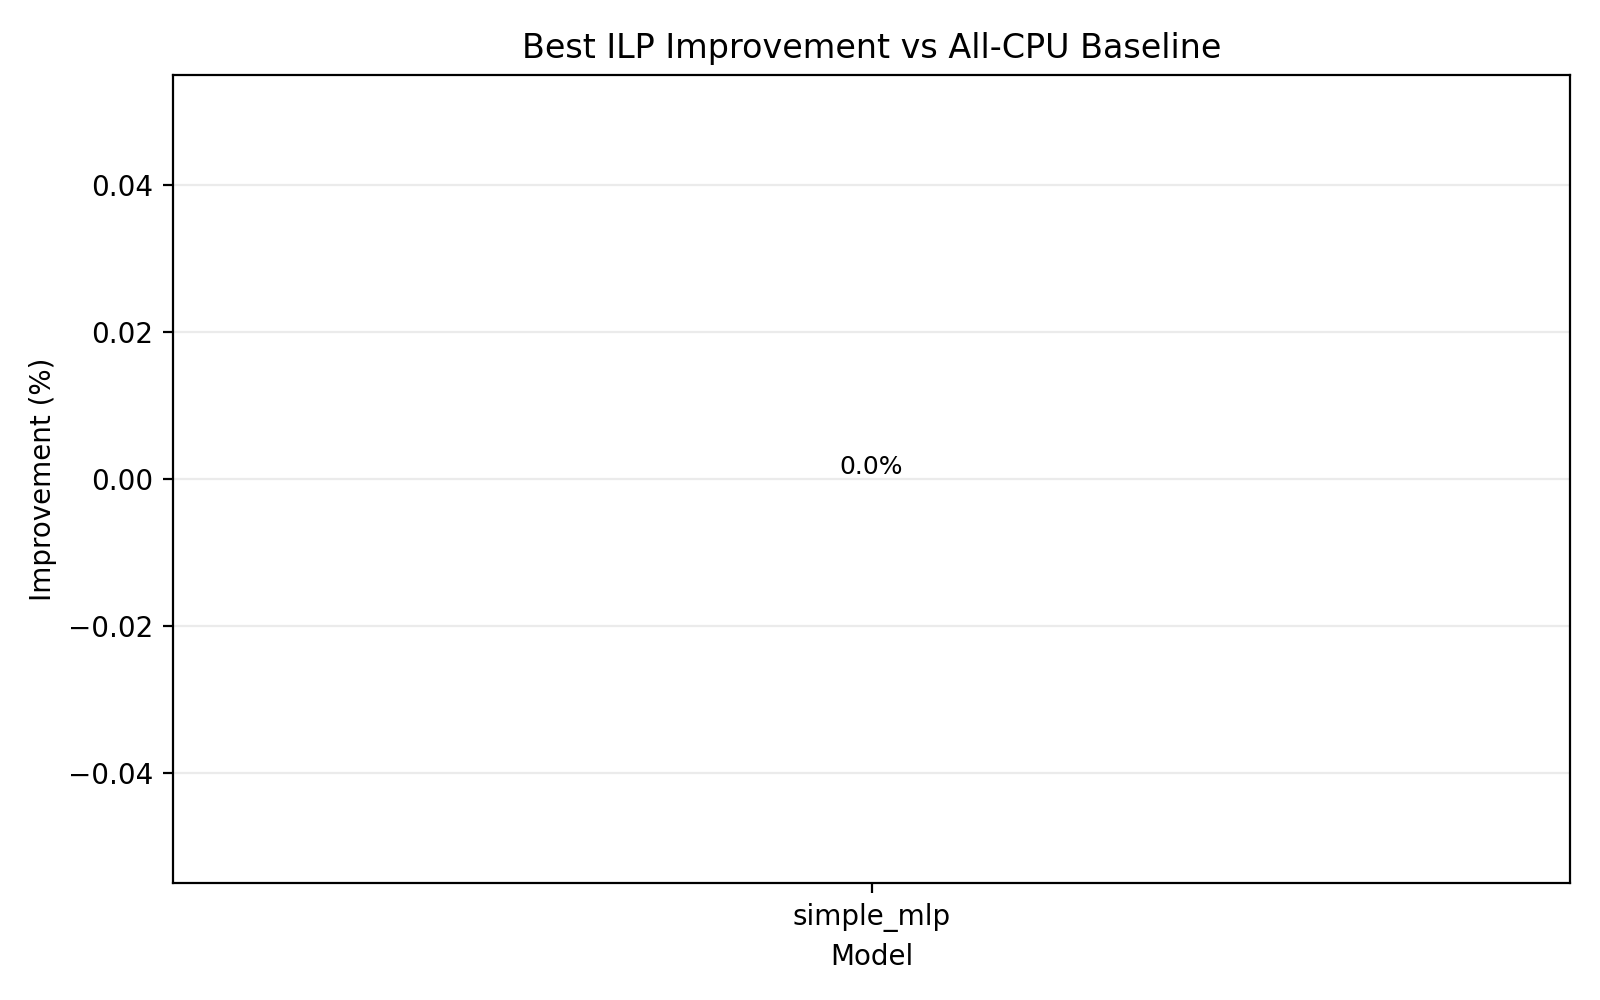
\includegraphics[width=0.82\textwidth]{../reports/ilp_results_phase1/best_ilp_vs_all_cpu_improvement.png}
\caption{Mejora porcentual del mejor plan ILP frente al baseline \code{all_cpu} en la campana de Fase 1. Esta figura resume la direccion favorable de la evidencia ILP antes del cierre empirico multi-servidor.}
\label{fig:ilp-vs-all-cpu}
\end{figure}

\section{7.3 Limites del modelo y del protocolo experimental}
El trabajo presenta limites que deben exponerse con precision. En el plano de modelado, la formulacion lineal no capta todas las no linealidades del hardware real, y el modelo alpha-beta de transferencia sigue siendo una aproximacion de primer orden. En el plano empirico, parte de la evidencia disponible procede todavia de mallas smoke o de casos controlados sobre modelos piloto, lo que restringe la generalizacion inmediata de ciertas conclusiones. En el plano experimental, la principal limitacion abierta es la ausencia de una campaña multi-servidor final completamente cerrada con al menos cinco replicas por configuracion en la malla canonica.

Existe ademas un limite narrativo que la tesis debe evitar: confundir madurez del software con amplitud de la validacion. El repositorio ya incorpora capacidades avanzadas como separacion forward/backward, persistencia de activaciones y prefetching; sin embargo, su explotacion estadistica amplia aun esta en curso. La conclusion correcta, por tanto, no es que el sistema este incompleto, sino que su cierre empirico de nivel doctoral todavia requiere una campaña final mas extensa.

\section{7.4 Lineas de trabajo futuro}
Las lineas de trabajo futuro se desprenden con claridad del estado actual del proyecto. La primera y mas inmediata es ejecutar la validacion multi-servidor definida en el protocolo metodologico del repositorio, consolidando un dataset heterogeneo que permita resolver ILP robusto inter-host y contrastar su transferibilidad real. La segunda es cerrar la comparacion sistematica prediccion-versus-observacion sobre una matriz final de modelos, no solo sobre casos piloto. La tercera es profundizar en la validacion de calidad final del entrenamiento, integrando accuracy, loss o metrica especifica de tarea como condicion de aceptacion tan relevante como tiempo o memoria.

Una cuarta linea, mas propiamente investigativa, consiste en enriquecer el modelo de costo con terminos no lineales o calibraciones por tramos que capturen saturacion y contencion de bus con mayor fidelidad. Una quinta es ampliar el estudio a familias de modelos mas grandes y a regimens de precision mas diversos, siempre que se preserve el mismo contrato de trazabilidad y admisibilidad metodologica. Estas extensiones no invalidan el nucleo actual del trabajo; lo prolongan hacia una agenda de investigacion posterior coherente con los limites ya identificados.

\section{7.5 Trazabilidad final entre afirmaciones y evidencia}
Una monografia doctoral sobre sistemas no se cierra adecuadamente solo con una enumeracion de aportes; debe explicitar la correspondencia entre cada afirmacion fuerte y la evidencia que la sostiene. La tabla siguiente resume esa relacion y fija, de manera deliberadamente conservadora, el alcance con el que cada resultado puede presentarse en esta etapa del manuscrito.

\begin{table}[t]
\centering
\caption{Trazabilidad entre afirmaciones nucleares del manuscrito y evidencia disponible.}
\label{tab:thesis-traceability}
\scriptsize
\setlength{\tabcolsep}{4pt}
\begin{tabularx}{\textwidth}{p{0.26\textwidth}X p{0.19\textwidth}}
\toprule
Afirmacion & Evidencia principal en el manuscrito & Alcance actual \\
\midrule
El proyecto produce coeficientes empiricos trazables por capa & Capitulo 4, Tabla~\ref{tab:profiling-artifacts}, Figura~\ref{fig:profiling-layer-costs}, Tabla~\ref{tab:profiling-example-simple-mlp} & Demostrado \\
La formulacion ILP supera baselines simples en casos consolidados & Capitulo 5, Figura de objetivo vs presupuesto y tablas de comparacion ILP & Demostrado en campanas focales \\
La solucion ILP puede transformarse en plan, simularse y ejecutarse & Capitulo 6, secciones de representacion, simulacion y ejecutor hibrido & Demostrado \\
Existe contraste predictivo en un caso controlado & Capitulo 6, Figura~\ref{fig:prediction-vs-observation} y Tabla~\ref{tab:prediction-vs-observation} & Demostrado en caso focal \\
Las extensiones duales y de prefetching tienen evidencia operacional & Capitulo 6, evidencia controlada de Fase 4 y discusion de extensiones avanzadas & Demostrado en validacion controlada \\
La tesis ya dispone de cierre empirico transversal multi-servidor & Protocolo multiservidor y discusion de limites en Capitulos 6 y 7 & Pendiente \\
\bottomrule
\end{tabularx}
\normalsize
\end{table}

La funcion de esta tabla no es solo resumir resultados, sino disciplinar la escritura final. Obliga a distinguir entre lo ya demostrado, lo demostrado solo en regimen focal y lo que aun debe completarse antes del deposito definitivo. Esa distincion es parte de la calidad epistemologica del manuscrito y protege la tesis frente a sobreafirmaciones.

\section{7.6 Valor doctoral del trabajo en su estado actual}
El valor doctoral del manuscrito, en su estado presente, no debe medirse exclusivamente por la cantidad de funcionalidad implementada ni por la longitud del documento, sino por la coherencia alcanzada entre problema, metodo y evidencia. A este nivel, la tesis ya exhibe un rasgo fuerte: ha transformado una intuicion de ingenieria sobre infrautilizacion de CPU y saturacion de memoria de GPU en una cadena argumental completa que incluye fundamento teorico, observacion empirica, formulacion declarativa, simulacion y validacion operacional. Ese encadenamiento no es trivial y constituye, por si mismo, una contribucion metodologica robusta.

Tambien es importante subrayar que el manuscrito ya se encuentra mas alla del estadio de propuesta conceptual. Existe un pipeline que produce artefactos, un modelo que resuelve decisiones no triviales, una semantica de plan que cierra el paso hacia simulacion y runtime, y evidencia focal de que las extensiones mas ambiciosas del alcance fuerte pueden materializarse de forma controlada. En consecuencia, la tesis no esta en una fase de mera promesa investigativa; se encuentra en una fase de consolidacion y ampliacion empirica. Esa diferencia debe quedar clara porque condiciona el modo en que se presentan tanto los aportes como las limitaciones.

Sin embargo, precisamente por esa madurez, el documento tiene la obligacion de sostener un criterio alto de prudencia interpretativa. Una tesis doctoral rigurosa no solo debe demostrar que puede hacer algo, sino delimitar con claridad donde termina la evidencia efectivamente disponible. El cierre multi-servidor, la ampliacion estadistica de la validacion y la consolidacion final de calidad del entrenamiento no son detalles secundarios: son las piezas que convertiran una demostracion fuerte de viabilidad metodologica en una afirmacion generalizable de alcance doctoral pleno. La honestidad con que el manuscrito marca esa frontera constituye una parte esencial de su calidad cientifica.

\section{7.7 Cierre final}
La pregunta que ha organizado esta investigacion puede formularse de manera simple: es posible redistribuir de forma cientificamente justificada el entrenamiento profundo entre CPU y GPU para aliviar la presion de memoria sin degradar el valor operacional del proceso. La respuesta que el manuscrito ya puede ofrecer es igualmente clara, aunque matizada: si, bajo un regimen metodologico que mida, modele, simule y observe la politica resultante. Esa condicionalidad no debilita la respuesta; la convierte en una tesis verificable y no en una intuicion optimista.

En ultima instancia, la contribucion del trabajo consiste en mostrar que la heterogeneidad computacional puede dejar de ser un trasfondo pasivo del entrenamiento para convertirse en objeto explicito de decision. Esa transformacion conceptual tiene implicaciones que exceden el caso concreto estudiado: invita a pensar el aprendizaje profundo no solo como optimizacion estadistica sobre datos y parametros, sino tambien como organizacion formal de recursos materiales escasos. En esa interseccion entre teoria del entrenamiento, sistemas heterogeneos y metodologia experimental se situa el nucleo intelectual de la monografia.

El cierre definitivo del doctorado exigira, todavia, ampliar y consolidar la evidencia transversal. Pero aun en su forma actual, el manuscrito ya fija una posicion fuerte: la particion heterogenea CPU-GPU no debe abordarse como una coleccion de ajustes aislados, sino como una politica formal, empiricamente calibrada y operacionalmente contrastable. Ese es el sentido profundo del trabajo y el criterio bajo el cual debe leerse su aportacion.
